\section{The Word is made Flesh}

\begin{quotex}
The Spirit blows wherever He wants, and you hear His voice, but you do not know where He is coming from nor where He is going; so it is with everyone born of the Spirit. \flright{\textsc{John 3:8}}

\end{quotex}

\begin{wrapfigure}{rt}{.22\textwidth}
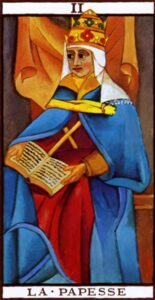
\includegraphics[scale=4]{a20221204TheWordismadeFlesh-img001.jpg} 
\end{wrapfigure}
The breath of the Spirit is the pure act of intelligence, arising from the Silence. So how do you hear his voice? We read in \emph{Meditations on the Tarot}:

\begin{quotex}
The pure act is unknowable in itself; it is only its reflection which makes it perceptible, comparable, and comprehensible; in other words, it is thanks to its reflection that we become conscious of it. 

\end{quotex}
The Spirit is active principle and the Virgin is the passive, reflecting principle, like the calm surface of a body of water. It takes the two conditions for the conscious experience of the Holy Spirit, or Kingdom of God. As Jesus tells Nicodemus in his nocturnal visit:

\begin{quotex}
Amen, amen, I say to you that a man cannot enter the Kingdom of God without being born of Water and the Spirit. \flright{\textsc{John, 3:5}}

\end{quotex}
Water represents consciousness. The reflection of the pure activity of the Holy Spirit will be distorted unless that consciousness is itself pure. Two qualities are necessary, one pertaining to the Mind, the other to the Will:

\begin{description}
\item[Virginal ]The Mind is free of false ideologies, beliefs, and dogmas. 
\item[Immaculate ] The Will is free of the cloudiness of the imagination, passions, and personal desires 
\end{description}
Reintegrated consciousness, the Kingdom of God, or the Primordial state requires a rebirth in the Spirit and Water, to be able to hear the Spirit and to reflect it accurately. This is how the Word expresses the Silence.

The Word is made flesh by the Holy Spirit through the Virgin Mary.

\begin{quotex}
Originally published on 16 Feb 2011.
\end{quotex}


\flrightit{Posted on 2022-12-04 by Cologero }
